\documentclass[12pt]{article}
%\usepackage[utf8]{inputenc}
%\documentclass[UTF8]{ctexart}
%\usepackage[UTF8, heading = false, scheme = plain]{ctex}
\usepackage{geometry}
%geometry{a4paper,scale=0.9}
\geometry{a4paper,left=1cm,right=1cm,top=1cm,bottom=2cm}
\usepackage{amsfonts}
\usepackage{color}
\usepackage{url}
%\usepackage{biblatex}
\usepackage{amsmath}
\usepackage{amssymb}
\usepackage{latexsym}
\usepackage{cite}
%\addbibresource{ref.bib}
%\bibliography{ref.bib}
\usepackage{caption}
\usepackage{graphicx, subfig}
\usepackage{float}
%\usepackage[fontset=ubuntu]{ctex}
%\usepackage{fontspec}
\usepackage{xeCJK}
%\usepackage[colorlinks,
%anchorcolor=black,
%citecolor=black]{hyperref}
%\setmainfont{SimSun}
\usepackage[section]{placeins}
\usepackage{enumitem}
\usepackage{framed}
\usepackage[framemethod=TikZ]{mdframed}
\usepackage{indentfirst}
\usepackage{setspace}%使用间距宏包
\linespread{1.5}
%\title{预备知识}
%\author{leolinuxer }
%\date{June 2020}

\begin{document}
%\maketitle

\section{Confusion Matrix}
Confusion Matrix 矩阵如下表所示:

\begin{table}[h]
\begin{center}  
\begin{tabular}{|l|l|l|}  
\hline  
预测值-实际值 & True & False \\ \hline  
True &	True Positive(真阳性) &	False Positive(假阳性)\\  \hline
False &	False Negative(假阴性) & True Negative(真阴性)\\  \hline
\end{tabular}  
\end{center}
\caption{Confusion Matrix} 
\end{table}

\section{各种率的定义}
正确率(Precision):
$$Precision = \frac{TP}{TP+FP}$$

真阳性率(True Positive Rate,TPR),灵敏度(Sensitivity),召回率(Recall):

$$Sensitivity = Recall= \frac{TP}{TP+FN}$$

真阴性率(True Negative Rate,TNR),特异度(Specificity):
$$Specificity = Recall= \frac{TN}{FP+TN}$$

假阴性率(False Negatice Rate,FNR),漏诊率( = 1 - 灵敏度):
$$ FNR = \frac{FN}{TP+FN}$$

假阳性率(False Positice Rate,FPR),误诊率( = 1 - 特异度):
$$ FPR = \frac{FP}{FP+TN}$$

\section{ROC 和 AUC \cite{ROC-AUC}}
\subsection{ROC}
对于分类器,或者说分类算法,评价指标主要有precision,recall,F-score等,以及这里要讨论的ROC和AUC。

ROC曲线:接收者操作特征曲线(receiver operating characteristic curve),是反映敏感性和特异性连续变量的综合指标,ROC曲线上每个点反映着对同一信号刺激的感受性。下图是一个ROC曲线的示例:

\begin{figure}[ht]
  \centering
  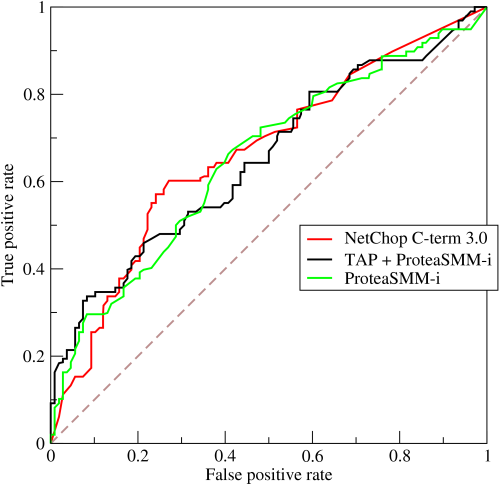
\includegraphics[width=.5\textwidth]{fig/ROC_example.png} %1.png是图片文件的相对路径
  \caption{ROC曲线示意} %caption是图片的标题
  \label{ROC_example} %此处的label相当于一个图片的专属标志,目的是方便上下文的引用
\end{figure}

ROC 曲线的横纵坐标分别为:

横坐标:1-Specificity,伪正类率(False positive rate, FPR),预测为正但实际为负的样本占所有负例样本的比例(负例中预测错了的比例);

纵坐标:Sensitivity,真正类率(True positive rate, TPR),预测为正且实际为正的样本占所有正例样本的比例(正例中预测对了的比例)。

在一个二分类模型中,假设采用逻辑回归分类器,其给出针对每个实例为正类的概率,那么通过设定一个阈值如0.6,概率大于等于0.6的为正类,小于0.6的为负类。对应的就可以算出一组(FPR,TPR),在平面中得到对应坐标点。随着阈值的逐渐减小,越来越多的实例被划分为正类,但是这些正类中同样也掺杂着真正的负实例,即TPR和FPR会同时增大。阈值最大时,对应坐标点为(0,0),阈值最小时,对应坐标点(1,1)。

\subsection{AUC(Area Under Curve)}
AUC (Area Under Curve) 被定义为ROC曲线下的面积,显然这个面积的数值不会大于1。又由于ROC曲线一般都处于y=x这条直线的上方(如果不是,那么可以交换阈值上下对应的分类,即可得到更好的分类结果),所以AUC的取值范围一般在0.5和1之间。使用AUC值作为评价标准是因为很多时候ROC曲线并不能清晰的说明哪个分类器的效果更好,而作为一个数值,对应AUC更大的分类器效果更好。

\subsection{为什么使用ROC曲线}
既然已经这么多评价标准(如precision-recall 等),为什么还要使用ROC和AUC呢?因为ROC曲线有个很好的特性:当测试集中的正负样本的分布变化的时候,ROC曲线能够保持不变。在实际的数据集中经常会出现类不平衡(class imbalance)现象,即负样本比正样本多很多(或者相反),而且测试数据中的正负样本的分布也可能随着时间变化。下图是ROC曲线和Precision-Recall曲线的对比:

\begin{figure}[ht]
  \centering
  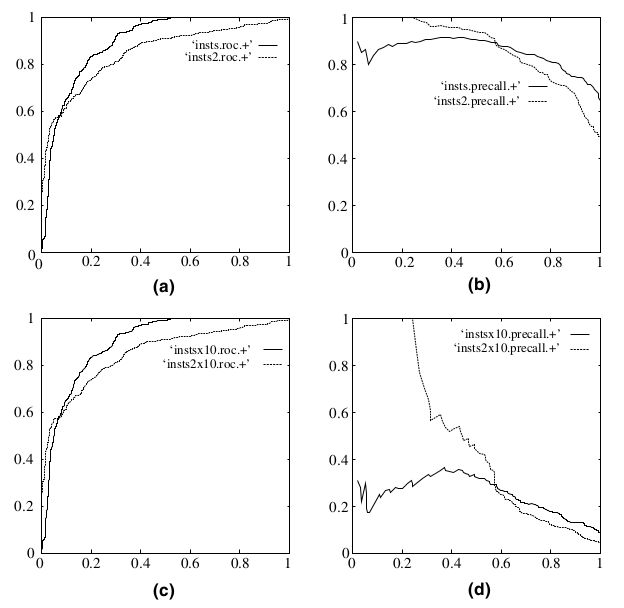
\includegraphics[width=.8\textwidth]{fig/ROC_vs_Precision_Recall.png} %1.png是图片文件的相对路径
  \caption{ROC vs Precision-Recall} %caption是图片的标题
  \label{ROC_vs_Precision_Recall} %此处的label相当于一个图片的专属标志,目的是方便上下文的引用
\end{figure}

在上图中,(a)和(c)为ROC曲线,(b)和(d)为Precision-Recall曲线。(a)和(b)展示的是分类其在原始测试集(正负样本分布平衡)的结果,(c)和(d)是将测试集中负样本的数量增加到原来的10倍后,分类器的结果。可以明显的看出,ROC曲线基本保持原貌,而Precision-Recall曲线则变化较大。

\subsection{精确率、准召率、F1 值 各自的优缺点\cite{Compare_P_R_F1_ROC_AUC}}

\subsubsection{精确率 Accuracy}
Accuracy 是最常见也是最基本的evaluation metric。但在binary classification 且正反例不平衡的情况下,尤其是我们对minority class 更感兴趣的时候,accuracy评价基本没有参考价值。什么fraud detection(欺诈检测),癌症检测,都符合这种情况。举个栗子:在测试集里,有100个sample,99个反例,只有1个正例。如果我的模型不分青红皂白对任意一个sample都预测是反例,那么我的模型的accuracy是正确的个数/总个数 = 99/100 = 99\%。你拿着这个accuracy高达99\%的模型屁颠儿屁颠儿的去预测新sample了,而它一个正例都分不出来,有意思么……也有人管这叫accuracy paradox。

\subsubsection{precision 和 recall}
准招率是比 Accuracy 更有用的metric。

recall是相对真实的答案而言: true positive / golden set 。假设测试集里面有100个正例,你的模型能预测覆盖到多少,如果你的模型预测到了40个正例,那你的recall就是40\%。

precision是相对你自己的模型预测而言:true positive /retrieved set。假设你的模型一共预测了100个正例,而其中80个是对的正例,那么你的precision就是80\%。我们可以把precision也理解为,当你的模型作出一个新的预测时,它的confidence score 是多少,或者它做的这个预测是对的的可能性是多少。

一般来说,鱼与熊掌不可兼得。如果你的模型很贪婪,想要覆盖更多的sample,那么它就更有可能犯错。在这种情况下,你会有很高的recall,但是较低的precision。如果你的模型很保守,只对它很sure的sample作出预测,那么你的precision会很高,但是recall会相对低。

这样一来,我们可以选择只看我们感兴趣的class,就是minority class的precision,recall来评价模型的好坏。

\subsubsection{F1-score}
F1-score 就是一个综合考虑precision和recall的metric: 

\begin{align*}
F1-score &= \frac{2}{1/precision + 1/recall}\\
     &= 2 * precision * recall / (precision + recall) 
\end{align*}

可以看出,F1-score是 precision 和 recall 的调和平均数(调和平均数(harmonic mean)又称倒数平均数,是总体各统计变量倒数的算术平均数的倒数。$H_n = n/\sum_{i=1}^n\frac{1}{x_i} = \frac{n}{\frac{1}{x_1} + \frac{1}{x_2} + \cdots + \frac{1}{x_n}}$)

如果两个模型,一个precision特别高,recall特别低,另一个recall特别高,precision特别低的时候,F1-score可能是差不多的,也不能基于此来作出选择。

%\printbibliography
\bibliography{../ref}
\bibliographystyle{IEEEtran}
\end{document}
